
\documentclass[conference]{IEEEtran}

\usepackage{graphicx}
\usepackage{stfloats}
\usepackage{color, colortbl}
\definecolor{Grey}{rgb}{0.90,0.90,0.90}

\begin{document}
\title{Synthetic Sympatric Speciation\\ Through Meiotic Inheritance}

\author{\IEEEauthorblockN{William Booker}
\IEEEauthorblockA{
School of Computer Science\\
University of Oklahoma\\
Norman, OK 73072\\
Email: william@thebookers.net}
\and
\IEEEauthorblockN{Dean Hougen}
\IEEEauthorblockA{
School of Computer Science\\
University of Oklahoma\\
Norman, OK 73072\\
Email: hougen@ou.edu}}

\maketitle
\begin{abstract}
Speciation is a critical process in both evolutionary science and machine learning. It helps us understand the development of life on Earth and can improve genetic algorithms' ability to find global maximums. In recent years, there has been considerable effort to understand this elusive process and uncover new techniques to simulate it. While there are many approaches for doing so, few examine one of the most important features of any genetic system: inheritance. This paper seeks to address this shortcoming and demonstrate how minor changes to a population's inheritance mechanism can radically alter a it's ability to speciate. Specifically, we look at how simulated meiotic inheritance with complete genetic dominance can significantly improve a population's divergent capability, even in absence of other speciation pressures. 
\end{abstract}

\section{Introduction}

Speciation describes the natural tendency for homogeneous populations to split and form discrete groups through the continuous process of evolution. \cite{SPBOOK} It underpins our understanding of biology and it is fundamental to the development of life on this planet. Additionally, speciation shows promise in the realm of artificial intelligence, as a mechanism by which to narrow in on optimal results in multi-modal solution spaces.

Evolutionary biologists define two distinct types of speciation: allopatric speciation, where isolated populations acquire new traits independently, and sympatric speciation, where a single population diverges over time. For our purposes, we are mostly concerned with sympatric speciation, as it has significant untapped potential for improving genetic algorithms. While there are many methods for inducing a type of allopatric speciation in genetic algorithms, such as such as niching \cite{NICHING}, population topologies \cite{TOPOLOGIES}, and island models \cite{ISLAND}, these approaches require implicit assumptions about the solution space which must be explicitly tailored to each problem. Ideally we would like to find a more general solution, where the algorithm speciates correctly in a number of different environments. 

For our experiments in sympatric speciation, we chose to examine an evolutionary model designed by Mark Woener et al. as part of the paper \textit{Sexual Selection, Resource Distribution, and Population Size in Synthetic Sympatric Speciation}. In the paper, the researchers hypothesized that sexual selection may be key to inducing sympatric speciation, as it has the potential to isolate sub-groups within a population, which could then evolve different traits in a similar manner to allopatric speciation. To test this hypothesis, the researchers set up a 2x2 factorial study using a simulated population of finches. In the study, the researches created two different distributions of seeds, bimodal and uniform, and observed the differences in population dynamics between finches that utilized sexual selection and those that did not.

\begin{figure}[t]
    \centering
    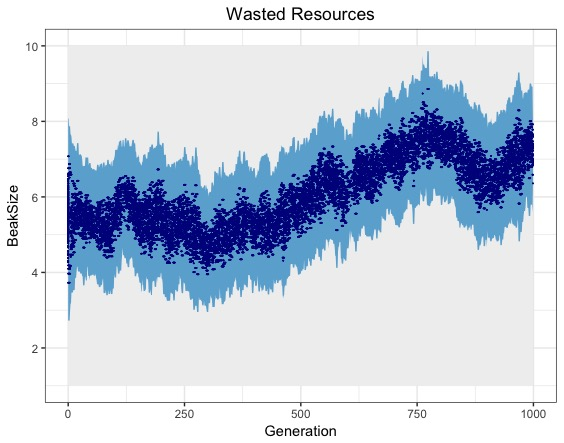
\includegraphics[width=\linewidth]{Data/FrontPage}
    \caption{Resource Waste in non-meiotic populations. Dark-blue represents populations members, light blue represents the population's effective feeding range, and grey represents wasted resources.}
    \label{fig:FrontPage}
\end{figure}

While the researchers successfully demonstrated that sexual selection could induce sympatric speciation in synthetic populations, they did not address how their results differed from speciation in the biological world. Specifically, in the simulation, when a population without sexual selection encountered a bimodal seed distribution, the population never expanded to cover both possible niches. This result is peculiar, as any species is highly incentivized to take advantage of all available niches in its environment. The convergence exhibited in the bimodal seed random mating scenario is known as bottlenecking, and typically only occurs in small, declining populations \cite{CHICKEN}. To see bottlenecking occurring in our large, healthy population suggests that there may be another factor at play, which may be enabling more phylogenetic divergence in biological populations.

\section{Hypothesis}

The cause of the population convergence in the bimodal seed random mating scenario is due to an oversimplification of genetic inheritance. Averaging the beak-sizes of the parents inhibits a population’s ability to maintain genetic diversity, which leads to population collapse in multi-niche environments. By introducing a biologically inspired meiotic inheritance model, the populations will exhibit higher levels of genetic diversity allowing them to exploit the full range of seeds in the random mating scenarios. 



\section{Overview}

This research can be divided into three phases: experimental replication, introduction of meiotic inheritance, and supplemental analysis. In the first phase (Experimental Replication), we successfully reproduced the simulation described in the \textit{Speciation} paper and validated the paper's results. In the second phase (Meiotic Inheritance), we modified the simulation to include a meiotic gene model and observed how the change affected the population's speciation potential. In the third phase (Supplemental Analysis), we modified the simulation to observe the effects of meitotic inheritance in a controlled environment. 

The results of our experiments are given in the form of population trees and extinction rates. The trees are organized into tables such that the columns represent gene structures and the rows represent the seed distributions and mating types. To test for statistical significance, we used a two-sample binomial test on the experimental and control proportions. The results of the first replication experiment are compared against the samples from the \textit{Speciation} paper, while the results for the remaining experiments were tested against our replicated values. 



\section{Experimental Replication}

The unmodified simulation is designed to replicate the simulation from the \textit{Speciation} paper. The details of this simulation are summarized in the following paragraphs. For a more in-depth analysis on the reasoning behind the choices made, please consult the original paper. 

The simulation consists of an island 100x100 units in size, filled with seeds and inhabited by a population of finches. Each finch has a known beak-size, age, gender, energy-level, and location. Each seed has a known size, energy-level and location.

The simulation begins by generating 400 finches with a roughly equal number of males and females. This initial population has a mean beak-size of 5.5 and a standard deviation of 0.5 \footnote{The \textit{Speciation} paper actually specifies a variance of 0.5, but the their data suggest that they actually used a standard deviation of 0.5.} (Gaussian distribution). These finches have their energy level set to zero and are randomly spread around the island. The island then undergoes an annual cycle consisting of a dry season and a mating season. This cycle repeats 1000 times during the simulation. 

The dry season lasts 100 days, and begins by spreading 5000 seeds randomly around the island. Each day, each bird has a chance to forage for food. The foraging is performed in a random order. Each bird searches a 10x10 plot of the island and consumes the first seed it finds that falls within one unit of its beak-size. This search costs the finch 0.1 units of energy. Any finch that has less than zero units of energy at the end of the day is declared dead and removed from the population.

The simulation accounts for two different distributions of seed sizes: bimodal and uniform. The bimodal distribution consists of two Gaussian distributions of 2500 seeds each; these distributions are centered at three and eight units, each with a standard deviation of 0.5 units. The uniform distribution consists of a single uniform distribution of 5000 seeds ranging from one to ten units in size. In both scenarios, a seed contains between zero and two units of energy (uniform distribution).

After the dry season ends, the remaining finches participate in that year's mating season. During the mating season, each female chooses a single male to mate with. Each male is only allowed to mate five times per breeding season. The simulation accounts for two types of mating: random mating, where females will choose any male from the population, and assorted mating, where females will only pick males within one unit of its beak-size. When presented with multiple possible mates, the female will choose between them at random. Mating produces a single offspring at the location of the mother. The child’s beak-size is an average of the beak-sizes of the parents plus a small Gaussian-random mutation (mean 0, standard deviation 0.2).

This process results in four discrete cases: bimodal seeds assorted mating (BSAM), bimodal seeds random mating (BSRM), uniform seeds assorted mating (USAM), and uniform seeds random mating (USRM). Each case is replicated 48 times to give insight into population extinction rates. 

We were highly successful at replicating the results from the initial experiment. These results are included in the appendix. 



\section{Meiotic Inheritance}

\subsection{Methods}

To test the impact of meiotic inheritance on population dynamics, we redesigned the inheritance method to mimic biological inheritance as closely as possible. We introduced this method using a two-step process, where we first introduced a new genetic structure and demonstrated that it had no impact on population dynamics before introducing full meiotic inheritance (see appendix). This additional step serves as a control study to demonstrate that the changes in population behavior result from the new inheritance method rather than the new genetic structure.

In the new genetic structure, each finch is equipped with two chromosomes, one from each parent. Each chromosome contains an array of one-hundred genes, each represented by a floating point value. The phenotype for a chromosome is determined by taking the sum of all its genes. In order to mimic the \textit{Speciation} paper’s initial population, the genes in the initial population are randomly chosen from a uniform distribution with a mean of 0.055 and a range of 0.245 \footnote{The mean of 0.055 and the range of 0.245 were determined mathematically. The final beak-size is equal to the average of two sums of 100 genes, or $(\sum_{i=1}^{200} x_{i})/2$. The distribution of the beak-sizes is normal by the central limit theorem. The mean is $(200 * 0.055)/2 = 5.5$, and the standard deviation is $\sqrt{\frac{1}{4}\sum_{i=1}^{200}Var(x_{i})} = 0.5$ where $Var(x_{i}) = \frac{0.245^2}{12}$.}. This model is a good fit for biological populations, as it represents how a single gene, Bmp4, is responsible for most of the variation in beak-sizes in real Darwinian finches \cite{BMP4}. 

When mating, the child receives one randomly selected chromosome from each of its parents. Each gene has a 10\% chance to mutate after the averaging process. When a gene is selected for mutation, we add a random value taken from a uniform distribution with a range of 0.310 and a mean of 0 \footnote{The running mutation range of 0.310 was determined empirically. We iteratively tested mutation ranges until the standard deviation of the change in beak-size consistently averaged at 0.2}. Our experiments use both a complete dominance (Cdom) and an incomplete dominance (Idom) model. In the complete dominance model, the larger of the two phenotypes is chosen for the finch's beak-size. In the incomplete dominance model, the two phenotypes are averaged to determine the beak-size. For the purposes of inheritance, this choice is arbitrary, as neither model affects the actual genetic material that is passed on to the child. 

\subsection{Results}

The results for the meiotic inheritance experiment are given in figure \ref{fig:EXP3} and table \ref{table:EXP3}. Columns one and three of figure \ref{fig:EXP3} represent the results from the gene model without meiotic inheritance. Columns two and four represent the introduction of meiotic inheritance. When testing for statistical significance, each dominance case is compared against the respective dominance case from the control study. 

\begin{figure*}
    \centering
    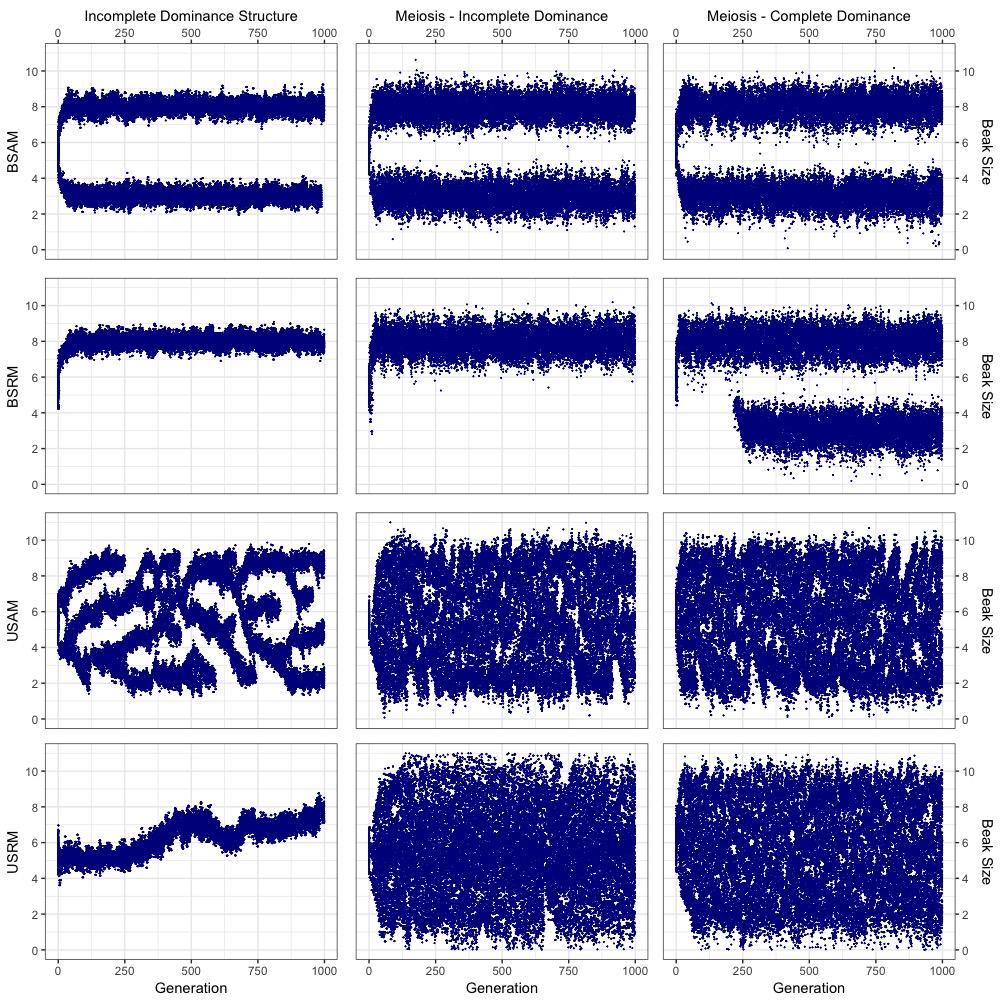
\includegraphics[width=\linewidth]{Data/EXP3}
    \caption{Introduction of Meiotic Inheritance}
    \label{fig:EXP3}
\end{figure*}

\begin{table*}
\centering
    \caption{Introducing Meiotic Inheritance: Bold is statistically significant at 1\%. Italics are statistically significant at 5\%.}
    \begin{tabular}{| p{3.00cm} *{4}{|c} |}
        \hline 
        \rowcolor{Grey}
        BSAM & Avg Idom & Meiosis Idom & Avg Cdom & Meiosis Cdom \\ \hline
        Speciation & 25 & 31 & 23 & 20 \\ \hline
        Partial Extinction & 23 & \textit{15} & 21 & 27 \\ \hline
        Extinction & 0 & 2 & 4 & 1 \\ \hline
        \rowcolor{Grey}
        BSRM & Avg Idom & Meiosis Idom & Avg Cdom & Meiosis Cdom \\ \hline
        Speciation & 0 & 1 & 0 & \textbf{33} \\ \hline
        Partial Extinction & 35 & 30 & 35 & \textbf{14} \\ \hline
        Extinction & 13 & 17 & 13 & \textbf{1} \\ \hline
        \rowcolor{Grey}
        USAM & Avg Idom & Meiosis Idom & Avg Cdom & Meiosis Cdom \\ \hline
        Branching & 41 & 37 & 41 & 41 \\ \hline
        Extinction & 7 & 11 & 7 & 7 \\ \hline
        \rowcolor{Grey}
        USRM & Avg Idom & Meiosis Idom & Avg Cdom & Meiosis Cdom \\ \hline
        Single Species & 24 & \textbf{44} & 34 & 40 \\ \hline
        Extinction & 24 & \textbf{4} & 14 & 8 \\ \hline
    \end{tabular}
    \label{table:EXP3}
\end{table*}

\subsection{Analysis}

The introduction of meiotic inheritance radically altered the results of the simulation. Rather than collapsing into narrow bands, each population rapidly expanded to cover the entire range of seed sizes. While the non-meiotic populations were limited to 2-unit thick population bands, the meiotic populations were stable at an arbitrary range. This trait allowed the meiotic populations to exploit the full range of available resources, particularly in the uniform seed distributions. 

Furthermore, both meiotic populations exhibited evidence of speciation in the BSRM scenario. The complete dominance case speciated thirty-three times, while the incomplete dominance case speciated once. This tendency suggests that in meiotic populations, speciation is possible even without sexual selection. The key to this discrepancy lies in the mechanism by which genetic information is passed on to the next generation. 

In the unaltered simulation, we averaged the beak-sizes of the parents to determine the beak-size of the child. This inheritance mechanism destroys important genetic diversity in the population. Barring mutation, any child produced using this method will have a beak-size between the beak-sizes of its parents. When scaled up, this effect causes each generation to cover a smaller range of beak-sizes than the generation that preceded it. Thus, over time, the species begins to coalesce around a single beak-size: population convergence. This effect is clearly demonstrated in the "No Mutation" experiment below. As the inheritance method pushes the population inwards, the high mutation rate pushes the population outwards, eventually reaching equilibrium at two-unit thick population bands. This equilibrium explains why the the population bands are the same width in the unaltered simulation regardless of niche size: the inheritance method is the force pushing the population inwards, not natural selection. This effect also explains why we don’t see speciation in the BSRM scenario for non-meiotic populations. Because the gap between the local maxima at three and eight are more than two units apart, there is no stable population that can contain both, forcing one niche to be abandoned.

Contrast this tendency with non-destructive meiotic inheritance, in which genetic information is passed unaltered from parent to child. By keeping the chromosomes the same between generations, meiotic inheritance protects the diversity of the population. There is no guarantee that a child’s beak-size will fall between that of its parents, so future generations can reassert genetic diversity that may not appear in the current distribution of phenotypes. By introducing meiotic inheritance, we removed the pressure towards convergence, allowing the population to diverge to cover the entire range of seed sizes. Because meiotic populations have no tendency for convergence, and are thus stable at an arbitrary range, they can exploit both population niches in the BSRM scenario.

\section{Supplemental Analysis}

\subsection{Overview}

While our initial experiment demonstrates the impact of meiotic inheritance, we developed two additional experiments to help support our analysis and address unexpected anomalies. First, we wanted to confirm our analysis regarding the convergent tendency of non-meiotic inheritance by removing mutation from the simulation and observing the effects. Second, we wanted to explain why incomplete dominance resulted in significantly fewer speciation events than complete dominance in the BSRM scenario. 

For simplicity, in these experiments, we made two changes to the simulation. First, rather than testing all population conditions, we only looked at the meiotic population conditions and one non-meiotic population condition in the BSRM scenario. Second, we reduced the initial population size from 400 down to 40 to help smooth out the initial population collapse and subsequent rebound that appeared in our initial experiments.



\subsection{No Mutation}

\begin{figure*}[ht]
    \centering
    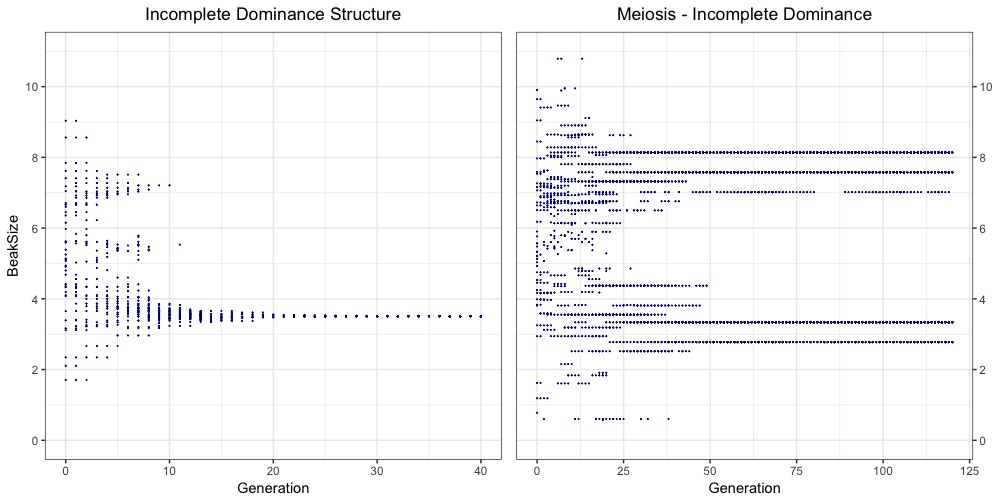
\includegraphics[width=\linewidth]{Data/EXP4}
    \caption{Removed Mutation}
    \label{fig:EXP4}
\end{figure*}

This experiment is designed to illustrate the convergent tendency of non-meiotic inheritance by removing the noise created by mutation. We achieved this effect by reducing the range of the running mutation rate from 0.310 to 0.00. We also quadrupled the initial mutation rate to 0.980 to give the starting population sufficient diversity to reach both niches. Both simulations utilize an incomplete dominance genetic structure. 

The results of this experiment are given in figure \ref{fig:EXP4} and represent the difference between non-meiotic and meiotic inheritance in the absence of mutation. As expected, the non-meiotic population exhibited clear signs of convergence, while the meiotic population retained population diversity throughout the duration of the simulation. 

Without the divergent pressure from mutation, the non-meiotic inheritance method immediately coalesced around a single beak-size. Each generation exhibited less diversity than the generation that proceeded it, eventually forcing the population to abandon one of the niches within a dozen generations. However, with meiotic inheritance, no such trend appeared. While some chromosomes did die out, the handful that survived were stable for the duration of the simulation. Some phenotypes even temporarily disappeared from the population, only to reemerge in later generations. These observations line up well with what we observe in real-world biological populations, which tend to exhibit a countable number of discrete phenotypes and demonstrate high levels of diversity despite extremely low mutation rates. While the simulated non-meiotic populations may look biologically accurate due to high mutation rates, this experiment demonstrates that they are actually governed by vastly different forces than real-world populations, making them unreliable for predicting biological behavior. 

\subsection{Initial Population}

\begin{figure*}
    \centering
    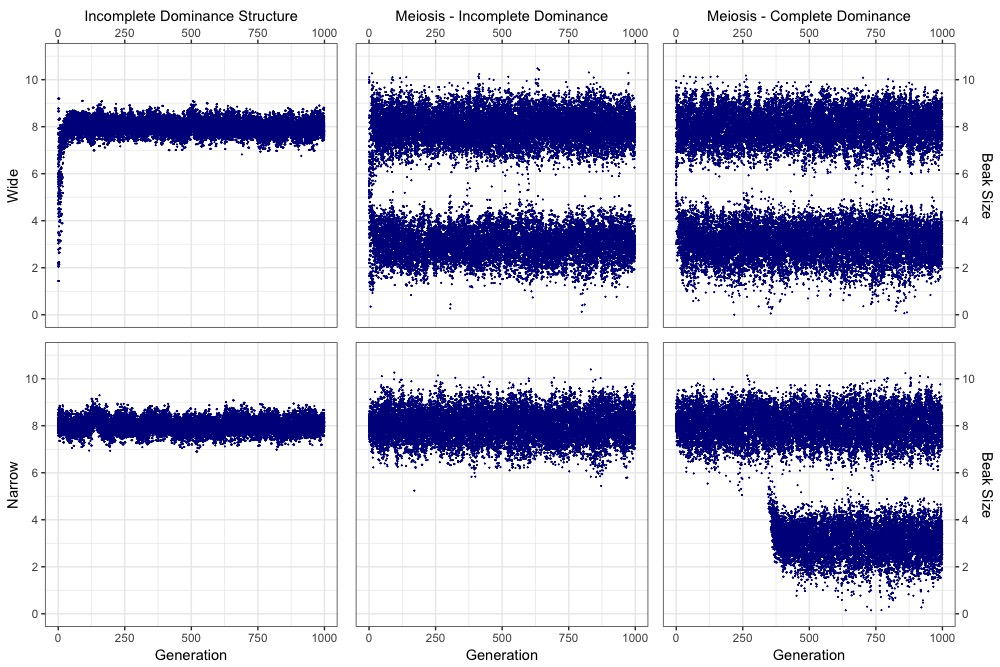
\includegraphics[width=\linewidth]{Data/EXP5}
    \caption{BSRM Scenario with Varying Initial Populations}
    \label{fig:EXP5}
\end{figure*}

Our initial experiment demonstrated that speciation is possible in meiotic populations in the BSRM scenario, but it did not address why complete dominance exhibited far higher rates of speciation than incomplete dominance. We believe that this phenomenon is caused by an unrelated property of genetic inheritance, which enables populations to bridge the evolutionary valley between the two optimums via genetic drift. In the case of complete dominance, only one chromosome is actually expressed, thus allowing the non-dominant chromosome to move through the low-fitness valley without reducing the organism’s evolutionary fitness. Eventually, these recessive chromosomes can wander into the second niche, and, when matched, they produce an individual capable of exploiting these untapped resources. With incomplete dominance, both chromosomes are expressed, so the population is unable to bridge the gap on its own. By masking the effect of one of the chromosomes, complete dominance acts as a multiplier on the mutation rate, allowing beneficial mutations to develop over the course of several generations rather than within a single individual. 

\begin{table}
\centering
    \caption{
        BSRM Scenario with Varying Initial Populations: Bold is statistically significant at 1\%. Italics are statistically significant at 5\%.}
    \begin{tabular}{| p{2.75cm} *{3}{|c} |}
        \hline
        \rowcolor{Grey}
        Wide & Avg Idom & Meiosis Idom & Meiosis Cdom \\ \hline
        Speciation & 0 & \textbf{39} & \textbf{43} \\ \hline
        Partial Extinction & 45 & \textbf{9} & \textbf{5} \\ \hline
        Extinction & 3 & 0 & 0 \\ \hline
        \rowcolor{Grey}
        Narrow & Avg Idom & Meiosis Idom & Meiosis Cdom \\ \hline
        Speciation & 0 & 0 & \textbf{12} \\ \hline
        Partial Extinction & 46 & 48 & \textbf{33} \\ \hline
        Extinction & 2 & 0 & 3 \\ \hline
    \end{tabular}
    \label{table:EXP5}
\end{table}

This experiment was designed to test this analysis. Assuming that the change in speciation rates was due to genetic drift through the low-fitness valley, we would expect that increasing the genetic diversity of the initial population would reduce its impact, while reducing the genetic diversity would increase it.

In this experiment, we changed the size of the initial population to see the effects on the extinction rates between incomplete dominance and complete dominance. For the first test, we widened the initial population to cover both niches by quadrupling the initial mutation rate to 0.980. In the second test, we reduced the initial population by halving the initial mutation rate to 0.1225 and moving the mean to 0.80. This change centers the population in the middle of the upper niche.

The results of the this experiment are given in figure \ref{fig:EXP5} and table \ref{table:EXP5}. The first column of figure \ref{fig:EXP5} represents the incomplete dominance case with the averaging inheritance method. The second and third columns represent meiotic inheritance with incomplete and complete dominance. When the population was widened, both meiotic populations exhibited high rates of speciation. When the population was narrowed, only the complete dominance case speciated, and the rate of speciation was dramatically reduced. The non-meiotic population exhibited no speciation events in either scenario. 

When the initial population was widened, incomplete dominance performed almost identically to complete dominance, with thirty-nine speciation events to forty-three. However, when the initial population was narrowed and confined to a single niche, there were no speciation events for incomplete dominance and twelve for complete dominance (the averaging method did not produce any speciation events in either condition). These results suggest that both incomplete dominance and complete dominance are equally effective in protecting genetic diversity in a population: complete dominance only performed better in our initial experiment because it added a method to bridge the low-fitness valley.



\section{Conclusion}

This research demonstrates the paramount importance of inheritance methods in biological simulations and genetic algorithms, and illustrates the need for increased scrutiny of an under-appreciated aspect of evolutionary computation.. A slight change in a population’s inheritance mechanism can radically alter the population dynamics, due to the potential introduction of strong evolutionary pressures. Obviously, for biological simulations, the inheritance process should mimic meiotic inheritance as closely as possible to avoid potential inaccuracy. While the applications for machine learning are less clear, we postulate that meiotic inheritance may have many advantages over assorted mating for inducing speciation in genetic algorithms.

First, meiotic speciation has an advantage in that it makes very few assumptions about the nature of the solution space. As demonstrated, non-meiotic inheritance has a tendency to collapse into narrow population bands that are only sustained by high mutation rates. If the mutation rate is too low, these narrow population bands run the risk of getting stuck local maxima before they are able to identify the optimal solution. This observation reduces the generalizability of the sexual selection technique, as the mutation rate must be hand-crafted to optimize for a given solution space. Meiotic inheritance avoids this drawback entirely by inhibiting population collapse during runtime. By keeping the population as wide as the niches will allow, meiotic inheritance is better protected against premature optimization.

Second, meiotic speciation has the potential to speed up the mating process, as random mating can be performed in O(n) time while sexual selection may take up to O($n^2$) time. Unlike with non-meiotic inheritance, where sexual selection was requisite for speciation, in meiotic inheritance, sexual selection is unnecessary, and in some cases, even counter effective \footnote{In our initial experiment, the speciation rate was higher in the BSRM complete dominance scenario than it was in the BSAM complete dominance scenario. This result stems from the fact that with assorted mating, the first member of new species is at a disadvantage, because its beak-size is too extreme to mate with the broader population.}. 

Third, meiotic inheritance has the ability to take advantage of a complete dominance structure, which we discovered is a powerful tool for exploring new niches without increasing the mutation rate. This ability is advantageous, as increasing mutation rates often result in the abandonment of good solutions \cite{TAGGING}. Meiotic inheritance is best equipped to utilize this technique, as the amount of genetic drift is not limited by the convergent tendency of the inheritance method.

Fourth, and perhaps most importantly, meiotic inheritance may prove useful in situations where the solution space itself is evolving over time. In this case, it's easy to imagine how premature optimization may trap a population in a niche from which it is unable to escape once it becomes unfavorable. Meiotic inheritance is well equipped to deal with such a scenario, given the high level of diversity and the ease with which it exploits new niches. When coupled with the additional search range offered through complete dominance, meiotic inheritance gains a major advantage over sexual selection in dynamic solution topographies. 

Despite these potential advantages, there are limitations to this technique that we would like to address in future work. The first issue is that our experiments use a dynamic population size, which, while biologically accurate, is uncommon in genetic algorithms. To expand the scope of this research, we would like to demonstrate an effective method by which to apply the benefits of meiotic inheritance with a static population size. Furthermore, many genetic algorithms that use an indirect encoding scheme, such as heuristic encoding \cite{CARLSON}, implicitly utilize a form of meiotic inheritance. In this case it may worth investigating the merits of using a non-meiotic inheritance method to improve population convergence. We hypothesize that for most solution spaces,  a combination of meiotic and non-meiotic inheritance would provide the optimal search. Methods for integrating both types of inheritance in the same population remains an area of future study. 

Finally, from a biological standpoint, it remains to be seen how sexual selection impacts sympatric speciation in the natural world. While we have demonstrated that the \textit{Speciation} paper’s results cannot be applied to biological populations, we have not established whether or not sexual selection is a key component of biological sympatric speciation. Our results should not be immediately extended to the biological world, because the speciation that we observed in meiotic populations in the BSRM scenario is likely very different from the speciation exhibited in biological populations. Specifically, for the purposes of this paper, we defined speciation as any set of visibly distinct populations exploiting separate niches. However, while useful for genetic algorithms, this definition is weaker than biological speciation, which typically requires that different species be reproductively isolated \cite{TEXTBOOK}. Thus, it could be argued that the distinct bands that arise in meiotic populations in the BSRM scenario do not actually comprise two distinct species, but rather a single species exploiting multiple niches. Further research is required to determine if sexual selection is required for this split population to diverge into separate species, or if there is another potential cause.

In summary, the findings of this paper are fourfold. One, we successfully replicated the results of the \textit{Speciation} paper and confirmed their findings. Two, we demonstrated that meiotic inheritance radically changes the behavior of the simulation, thus providing evidence against the \textit{Speciation} paper's biological conclusions. Three, we demonstrated that meiotic inheritance allows for speciation in multi-niche environments, which may have applications in evolutionary computation. And four, we demonstrated that complete dominance gives populations the opportunity to explore the low-fitness valley, even when the mutation rate is smaller than the expanse. 

\section{Appendix}

\subsection{Results}

The results from the experimental replication and our first control study are given in figure \ref{fig:EXP2} and table \ref{table:EXP2}. In figure \ref{fig:EXP2}, the first column represents the extinction rates given in the \textit{Speciation} paper and the second column represents our replicated results. The third and fourth columns represent the introduction of the new genetic structure, without meiotic inheritance. As expected, the results from our replication and control experiment closely match those from the initial paper. Specifically, we see high rates of speciation in the BSAM and USAM scenarios, and no speciation in the BSRM and USRM scenarios.

\begin{table}
\centering
    \caption{
        Experimental Replication and Introducing Gene Structure: Bold is statistically significant at 1\%. Italics are statistically significant at 5\%.}
    \begin{tabular}{| p{2.00cm} *{4}{|c} |}
        \hline
        \rowcolor{Grey}
        BSAM & Baseline & Replication & Avg Idom & Avg Cdom \\ \hline
        Speciation & 31 & 30 & 25 & 23 \\ \hline
        Partial Extinction & 17 & 15 & \textit{23} & 21 \\ \hline
        Extinction & 0 & \textit{3} & \textit{0} & 4 \\ \hline
        \rowcolor{Grey}
        BSRM & Baseline & Replication & Avg Idom & Avg Cdom \\ \hline
        Speciation & 0 & 0 & 0 & 0 \\ \hline
        Partial Extinction & 41 & 38 & 35 & 35 \\ \hline
        Extinction & 7 & 10 & 13 & 13 \\ \hline
        \rowcolor{Grey}
        USAM & Baseline & Replication & Avg Idom & Avg Cdom \\ \hline
        Branching & 35 & 37 & 41 & 41 \\ \hline
        Extinction & 13 & 11 & 7 & 7 \\ \hline
        \rowcolor{Grey}
        USRM & Baseline & Replication & Avg Idom & Avg Cdom \\ \hline
        Single Species & 35 & \textbf{23} & 24 & \textbf{34}\\ \hline
        Extinction & 13 & \textbf{25} & 24 & \textbf{14} \\ \hline
    \end{tabular}
    \label{table:EXP2}
\end{table}


\begin{figure*}
    \centering
    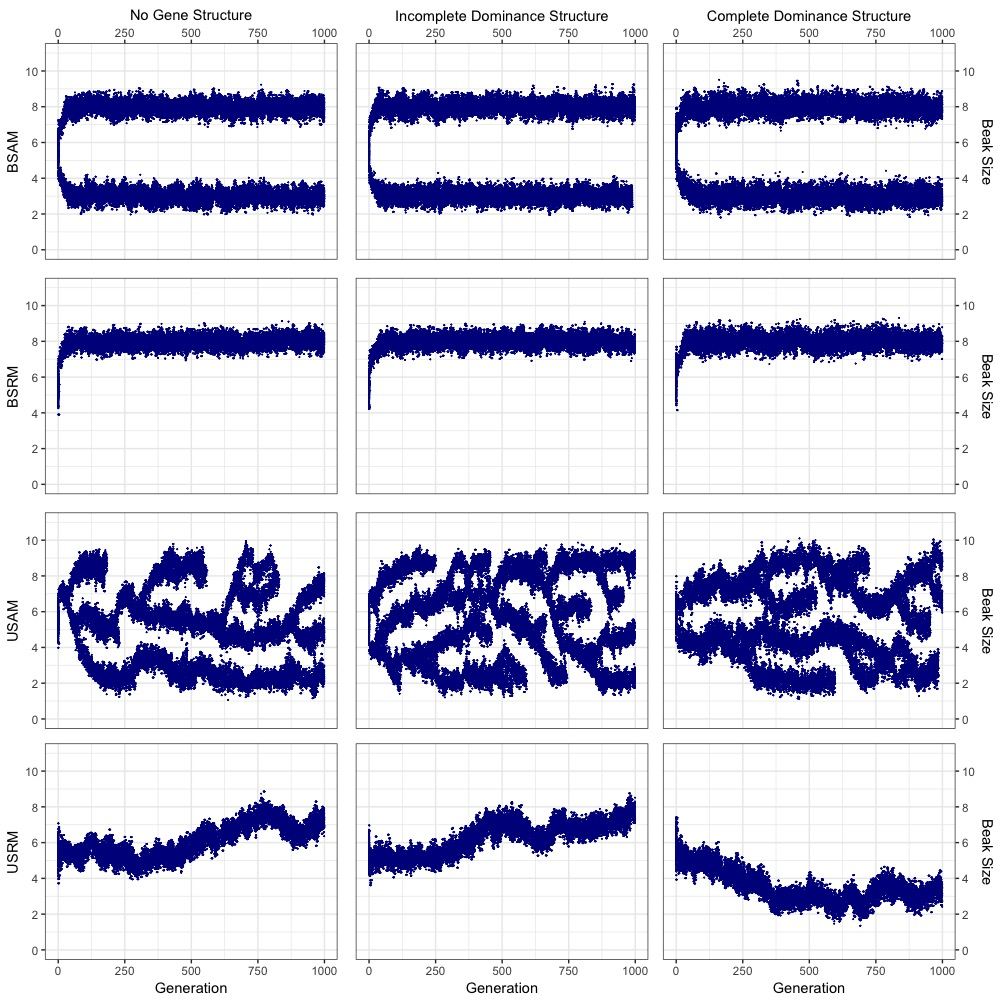
\includegraphics[width=\linewidth]{Data/EXP2}
    \caption{Introduction of Gene Structure}
    \label{fig:EXP2}
\end{figure*}

\subsection{Analysis}

In the BSAM, BSRM, and USAM cases, the population distributions, the widths of the population bands, and the number of extinction events lined up extremely well with what was described in the \textit{Speciation} paper. In the USRM scenario, the population distribution and the widths of the bands were correct, but there were significantly more extinction events than expected. We suspect that this anomaly might be due to a minor difference between our implementation and that of the initial experiment that was not covered in the original paper. Furthermore, it’s worth noting that we experienced another anomaly in the USRM scenario in the control experiment, suggesting that the extinction rates in this scenario might be unusually sensitive to minor changes in experimental setup. However, despite this anomaly, we are confident that we have successfully replicated the \textit{Speciation} paper’s results.

In the control study, we introduced the new genetic structure but kept the averaging method the same, then compared the results against our findings from the first experiment. As expected, the population trees and extinction rates closely matched our original results. Again, the only major variation was in the extinction rates for the complete dominance structure in the USRM scenario. We suspect that this variation may have been the result of the slight skewing of the phenotypes of the initial population, caused by the switch from incomplete dominance to complete dominance. Nevertheless, this experiment demonstrates that the new genetic structure had little impact on the behavior of the populations.

\bibliography{IEEEabrv}
\begin{thebibliography}{1}

\bibitem{BMP4}
Arhat Abzhanov.
\newblock Bmp4 and morphological variation of beaks in darwin's finches.
\newblock {\em Science}, 2004.

\bibitem{TEXTBOOK}
Niel~A. Campbell, Brad Williamson, and Robin~J. Heyden.
\newblock {\em Biology Exploring Life}.
\newblock Pearson, 2006.

\bibitem{SPBOOK}
Jerry~A. Coyne and H.~Allen Orr.
\newblock {\em Speciation}.
\newblock Sinauer Associates, 2004.

\bibitem{NICHING}
Jeffrey Horn, Nicholas Nafpliotis, and David~E Goldberg.
\newblock A niched pareto genetic algorithm for multiobjective optimization.
\newblock {\em IEEE}, 1994.

\bibitem{CHICKEN}
Harris A. Lewin Ronald L. Westemeier Jeffrey D. Brawn Ken N.~Paige Juan
  L.~Bouzat, Hans H.~Cheng.
\newblock Genetic evaluation of a demographic bottleneck in the greater prairie
  chicken.
\newblock {\em Conservation Biology}, 1998.

\bibitem{TOPOLOGIES}
Jayshree~A Sarma.
\newblock An analysis of decentralized and spatially distributed genetic
  algorithms.
\newblock {\em Bombay University}, 1998.

\bibitem{TAGGING}
William~M. Spears.
\newblock Simple subpopulation schemes.
\newblock {\em World Scientific}, 1994.

\bibitem{ISLAND}
Darrell Whitley, Soraya Rana, and Robert~B Heckendorn.
\newblock The island model genetic algorithm: On separability population size
  and convergence.
\newblock {\em Colorado State University}, 1998.

\bibitem{CARLSON}
FIXTHIS
\newblock FIXTHIS
\newblock {\em Colorado State University}, 1998.

\end{thebibliography}







% that's all folks
\end{document}


